\documentclass[Proceedings]{ascelike}
\NameTag{May. 1, 2018}

\usepackage{indentfirst} 
\usepackage{xcolor}
\usepackage{graphicx} 
\usepackage{booktabs}
\usepackage{amsmath}
\usepackage{setspace}
\usepackage{algorithm,algorithmic}
\usepackage{float}
\usepackage{subfigure}

\begin{document}

\title{THE IMMUNE NETWORK THEORY}
\author{
Shi Haixin, 21721245, Computer Science and Technology
}
\maketitle

\begin{abstract}
The immune network theory is a theory of how the adaptive immune system works, that has been developed since 1974 mainly by Niels Jerne and Geoffrey W. Hoffmann. This theory states that interactions between the V regions of antibodies play a key role in the regulation of the system. But the hypothesis did not spell out many details of how this might occur; that came later with the explicit network models that have been developed, including the Richter theory and the symmetrical network theory. These three theories inherit and develop each other. In this article, we introduced them in detail and presented their mathematical models. In addition, we also compared and summarized them. Finally, taking the environmental detection algorithm as an example, a specific application of the immune network theory is given.
\end{abstract}

\KeyWords{The immune network theory, the environmental detection algorithm.}

\section{1. Introduction}
Immunologists in the early 1970's were in the process of discovering a wealth of information about how the immune system worked. They had found that the system is eminently manipulable. They could take it apart, then put it back together, and it would work! The puzzle was to work out how it all works. Then Niels Jerne, the Director of the Basel Institute for Immunology, published the seminal papers that gave birth to the network way of looking at the system[1].
\par
Jerne's network hypothesis was a radical innovation. The essence of it was, paraphrased, "This idiotypic network exists, since if antibodies can recognize essentially anything, they can recognize the V regions of other antibodies. V-V recognition within the system cannot be avoided. I propose that immune system regulation involves V-V interactions in a fundamental way, and predict that understanding such interactions will be the key to understanding many immunoregulatory phenomena, including specific suppression." Previously each of the clones had been regarded as a separate entity; and now he was suggesting that they were all strongly interconnected. Recall that the first law of cellular immunology is clonal selection. Jerne introduced the second law of cellular immunology, which states that the regulation of the adaptive immune system involves interactions between V regions.
\par
The network hypothesis included the development of some new vocabulary. Jerne introduced the terms epitope, idiotope and paratope. Epitope, also called antigenic determinant, is the part of an antigen that is recognized by the immune system, specifically by antibodies, B cells, or T cells. Idiotope is the unique set of antigenic determinants (epitopes) of the variable portion of an antibody. Paratope, also called antigen-binding site, is a part of an antibody which recognizes and binds to an antigen. 
\par
Besides, the number two played an important, almost metaphysical role in Jerne's thinking; he stressed a perceived importance of "dualisms". For example, there were two main kinds of cells involved (T cells and B cells) and two main kinds of interactions (stimulation and suppression). But as network theory subsequently developed, the two main kinds of interactions were to become three with the substitution of inhibitory (blocking) and killing interactions for the mechanistically less well defined "suppressive" interactions (beginning with the Richter model described below), and the two main classes of cells were to become three when non-specific accessory cells were included.

\section{2. Jerne's network hypothesis}

\subsection{2.1. Jerne's model of the network}
\begin{figure}
\centering
    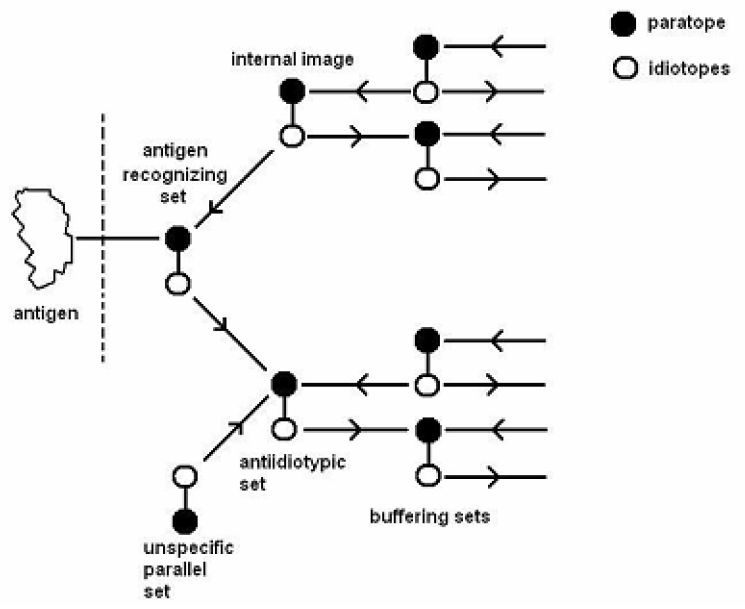
\includegraphics[scale=0.5] {img/network_model_jerne.png}
    \caption{Jerne’s model of the network}
\end{figure}
Each antibody/clone has V regions that include a recognizing part (paratope) and parts that can be recognized by other antibodies/clones (idiotopes). The antigen recognizing set is stimulated by both an epitope (antigenic determinant) of the antigen and idiotopes of antibodies/clones that are an internal image of the epitope (mimic the epitope in that they stimulate the antigen recognizing set). FIG. 1 shows only the stimulatory interactions. For each stimulatory interaction there is a suppressive interaction in the opposite direction. The interaction between the antigen and the recognizing set is of course asymmetric; the antigen stimulates the antigen recognizing set and the antigen recognizing set eliminates the antigen.
\par
It is assumed in this model that, as a first approximation, the interaction between the recognizing set and the internal image set is similarly asymmetric; the internal image set stimulates the antigen recognizing set while the antigen recognizing set suppresses or eliminates the internal image set. As a result of this asymmetry, there is another population that interacts with the antigen recognizing set called the antiidiotypic set, with the opposite interactions. The antigen recognizing set stimulates the antiidiotypic set, and the antiidiotypic set suppresses or eliminates the antigen-specific set. The asymmetry furthermore leads to the expanding definition of further sets that are either stimulatory or suppressive for each of the internal image set and the antiidiotypic set (buffering sets) including an unspecific parallel set that has idiotopes similar to the antigen recognizing set and paratopes that recognize different antigens. Each arrow denotes stimulation of paratope(s) by idiotope(s); not explicitly shown is suppression or elimination in the opposite direction[2].
\par
Jerne’s model was ingenious in that it appeared to resolve some important paradoxes, but mathematical modelling has shown that the details have to be different. My initial attempts to mathematically model the interactions as illustrated in the figure showed that the system typically oscillates, rather than exhibit multiple stable steady states, as is needed for a system that has memory.
 
\subsection{2.2. The first mathematical model}
Jerne recognized that mathematical modelling would have to play a role in the development of a more detailed immune network theory. He proposed the following differential equation to describe the dynamics of a typical clone consisting of L cells (lymphocytes)[3]:
\begin{equation}{
    \frac{dL}{dT}= \alpha -\beta L+\sum_{i=1}^{N}\varphi (E_{i},K_{i},t)-L\sum_{j=1}^{n}\psi (I_{j},K_{j},t)}
\end{equation}
\par
There are four terms in the differential equation for L. These correspond to non-specific influx (\boldmath$\alpha$), natural death (\boldmath$-\beta L$), a stimulation term due to all the clones with idiotopes that fit into the paratopes of the clone (the first summation term) and a killing term due to all the clones with paratopes that recognize the idiotopes of the receptors of the clone (the second summation term). This equation incorporates the asymmetry between idiotopes and paratopes shown in FIG.1. No analysis of this equation has been published, and as it stands the system is incompletely specified. Jerne later further formalized the distinction between the antiidiotypic set and the internal image set by calling the former \boldmath$Ab2\alpha$, and the latter \boldmath$Ab2\beta$[4]. 

\subsection{2.3. Limitations of the Jerne model}
While Jerne's model was a huge conceptual advance, he candidly recognized it's limitations. It is interesting to evaluate Jerne's model from the point of view of the five criteria for a good theory:
\begin{itemize}
\item
Simplicity: When Jerne published the theory, many immunologists wailed, "It's too complicated." However, complexity and simplicity are however in the eye of the beholder, FIG.1 has an important simplicity, namely it is constructed according to the simple (even if ultimately erroneous) rule that epitopes stimulate paratopes, and paratopes suppress epitopes. This would later be replaced by the even simpler concept known as “first symmetry”, in which the distinction between paratopes and idiotopes largely evaporates.
\item
Scope: The potential scope of the network hypothesis in general was enormous, since it provided a fundamentally new way of looking at immunoregulatory phenomena. As listed above, the phenomena that the Jerne model tentatively explained is impressive. The limitations in scope were also candidly acknowledged. 
\item
Predictions: The Jerne model did not make explicit new predictions. The Richter theory and the symmetrical network theory that followed were more explicit with respect to the underlying mechanisms and consequently had stronger predictive power. 
\item
Resolution of Paradoxes. The model provided explanations for several phenomena that are paradoxical in the context of a non-network clonal selection point of view. As mentioned, these included the phenomena of low zone tolerance, antigenic competition. 
\item
Rigor. The proposed mechanisms were more at a handwaving level than at a rigorous level with some mathematical modelling.
\end{itemize}

\section{3. The Richter theory}

\subsection{3.1. The model of Richter theory}
It did not take long for mathematical biologists to take up the challenge of translating Jerne's network hypothesis into a more concrete model or theory, with more explicit postulates about how the system might work. The first detailed model (or "theory") based on the network hypothesis was developed by Peter Richter of the Max Planck Institute for Biophysical Chemistry in Göttingen, Germany[5]. The aim of the theory was to explain the fact that either low or high doses of antigen can induce unresponsiveness ("high dose tolerance" and "low dose tolerance"), while intermediate doses induce an immune response. 
\begin{figure}
\centering
    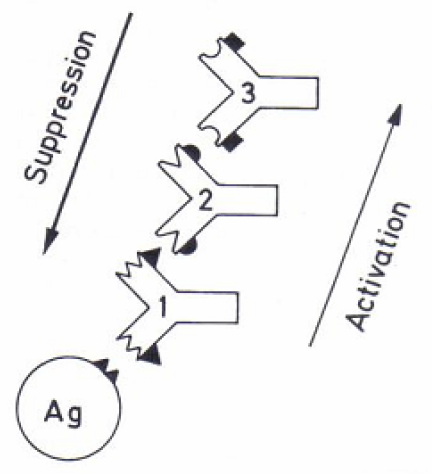
\includegraphics[scale=0.5] {img/network_model_richter.png}
    \caption{The model of Richter theory}
\end{figure}
\par
What we can see in FIG.2 is the chain Ab-1, Ab-2 and Ab-3 of Richter’s model. Ab-1 is the antigen recognizing set, Ab-2 is the antiidiotypic set, and Ab-3 is anti-antiidiotypic clones. The interactions are again asymmetric, with a clear distinction being made between paratopes that recognize and idiotopes that are recognized. All idiotypic interactions are assumed to be initially sub-threshold. The levels of the internal image set and the unspecific parallel set of the Jerne model consequently remain sub-threshold in this model, since they can only be suppressed by any increase in Ab-1 and Ab-2 respectively. The introduction of thresholds thus results in the more complex two-dimensional diagram of interactions of the Jerne model being simplified to become a one-dimensional chain, consisting of idiotype, antiidiotype, anti-antiidiotype, and so on[5] .

\subsection{3.2. Modes of responsey}
In the Richter theory, injection with various amounts of an antigen causes a wave of activation that propagates to various extents along the chain of specific cells Ab-1, Ab-2, Ab-3, and so on. A small dose may initially cause proliferation of just the Ab-1 lymphocyte population. When the Ab-1 population reaches a certain threshold level (the stimulation threshold) it causes proliferation of the Ab-2, and when Ab-2 reaches a different level, the threshold level for killing, Ab-2 cells and/or antibodies kill the Ab-1 cells (FIG.3(a)). The Ab-2 cells then persist at a level above the killing threshold level and below the threshold needed for stimulation of Ab-3. This requires that the killing threshold be lower than the stimulation threshold. This sequence of events was hypothesized to account for the phenomenon of low dose tolerance.
\par
An injection with a larger dose of antigen in this model causes an immune response, consisting of a wave of activation proceeding one step further along the chain. Then Ab-3 eliminates Ab-2, leaving Ab-1 free to respond to stimulation by the antigen, unencumbered by any restraining regulatory influence of Ab-2 (FIG.3(b)).
\par
An even larger dose of antigen takes the wave of activation one step further still, activating Ab-4, that eliminates Ab-3, permitting Ab-2 to emerge and eliminate Ab-1. Since the antigen-specific clones are eliminated, the animal cannot make antibodies, and we again have tolerance; in this case "high dose tolerance." (FIG.3(c)).
\begin{figure*}[!t]
\centering
\subfigure[] {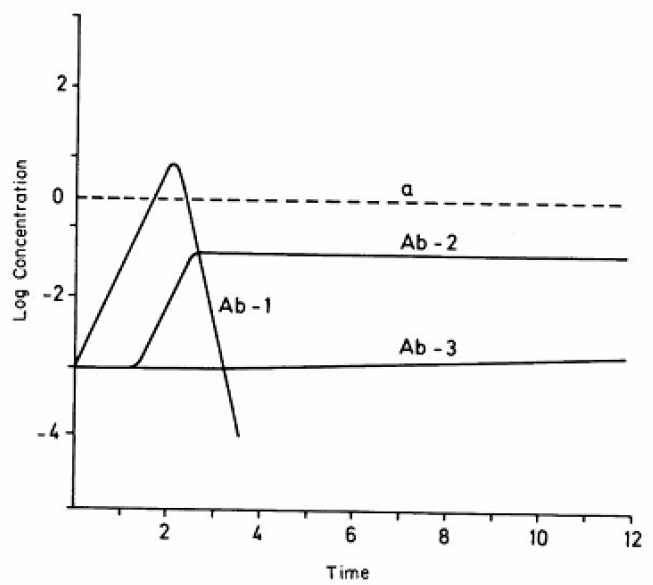
\includegraphics[height=2in,width=1.85in]{img/low_dose_tolerance.png}}
\subfigure[] {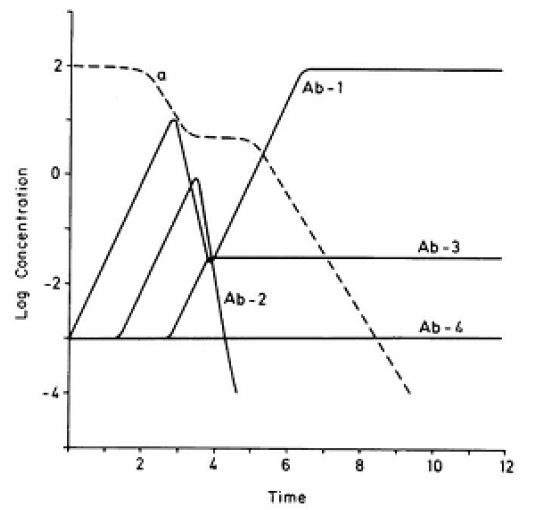
\includegraphics[height=2in,width=1.85in]{img/immune_response.png}}
\subfigure[] {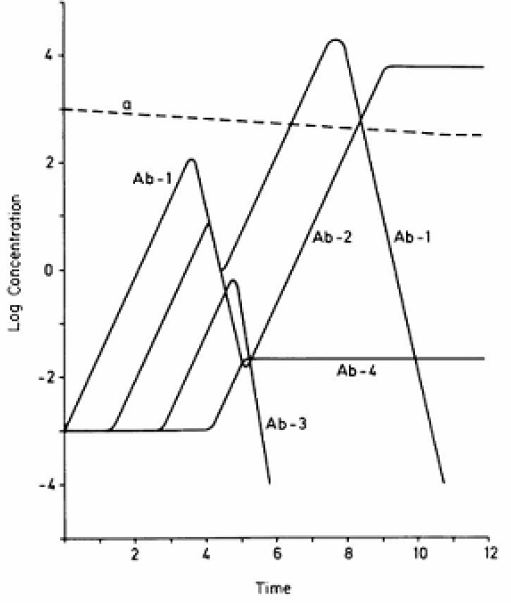
\includegraphics[height=2in,width=1.85in]{img/high_dose_tolerance.png}}
\caption{ Different dose of tolerance in the Richter theory}
\end{figure*}
\par
When Richter first mathematically modelled the simple chain of interactions shown in Figure 3-1, he found that he was unable to obtain both low dose tolerance and the immune response; a reasonable mathematical model resulted only in the dynamical behavior he was seeking for low dose tolerance (personal communication). This led him to add inhibitory interactions, as shown in FIG.4.
\begin{figure}
\centering
    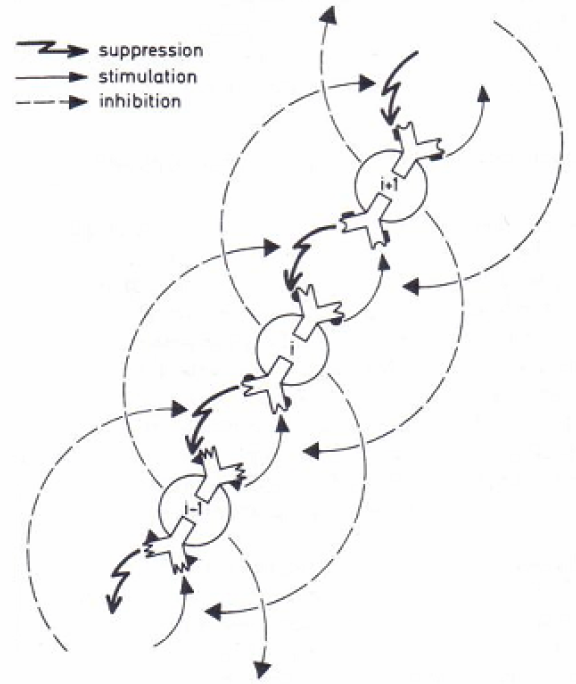
\includegraphics[scale=0.4] {img/Improved_network_model.png}
    \caption{The improved model of Richter theory}
\end{figure}

\subsection{3.3. Richter's mathematical model}
Richter translated the above ideas into differential equations, and FIG.3 (a) to (c) are obtained by integrating his equations, which appear below. Richter used dimensionless variables \boldmath$S_{i}$ for the size the clones, these variables can be interpreted as the product of a concentration and an affinity. The Richter equations have the form:
\begin{equation}{
    \frac{dS_{i}}{dt}=\frac{1}{\tau _{b}}f(S_{i-1},S_{i},S_{i+1})S_{i}-\frac{1}{\tau _{d}}g(S_{i-1},S_{i},S_{i+1})S_{i}}
\end{equation}
\par
The first term describes birth, the second death. The functions f and g are threshold functions that for the rate of change of \boldmath$S_{i}$ depend on \boldmath$S_{i-1}$, \boldmath$S_{i}$ and \boldmath$S_{i+1}$. The thresholds play a key role in the model. Jerne had suggested that network interactions are operative before the antigen arrives. This is the case in the symmetrical network theory, but was not the case in Richter's model because of the thresholds. In Richter's model the V-V interactions are all sub-threshold prior to the appearance of the antigen.
\par
\boldmath$\tau _{b}$ and \boldmath$\tau _{d}$ are birth and death time constants. The functions f and g are structured to model the thresholds that are inherent in the theory, with minimum values of 0 and maximum values of 1. In the case of the function f there are thresholds for stimulation (\boldmath$S_{i-1}$ dependence) and for inhibition of stimulation (\boldmath$S_{i+1}$ dependence). There is also a dependence on \boldmath$S_{i}$, which accounts for the fact that the amount of stimulation depends on how many cells there are to stimulate or kill (buffering dependence).

\subsection{3.4. Achievements of the Richter theory}
The Richter model was the first one that successfully addressed what the theorists of the time regarded as the most interesting system-response behavior, it can reasonably be called a theory. It achieved several things. Firstly, it showed that Jerne's network concept could be reduced to manageable proportions, which was something about which Jerne himself had not been optimistic. Secondly, the Richter theory showed that there are three basic types of specific interactions which are important for such models - stimulation, inhibition (blocking) and elimination (killing). Thirdly, it illustrated a potential importance of thresholds in stabilizing the immune system. In conclusion, the publication of the Richter theory was thus a big step towards making the network concept plausible.

\section{4. The symmetrical network theory}
In the third section I described the Richter theory, the first mechanistic theory to be developed based on Jerne's immune network hypothesis. In the fourth section I now describe a second mechanistic immune network theory called the symmetrical network theory, that incorporates symmetric interactions between idiotypes and antiidiotypes. The first paper was published by Hoffman in 1975, at a time when the dominant point of view favored asymmetric rather than symmetric V-V interactions[6]. Due to space limitations, I will briefly introduce its basic ideas here.
\begin{figure}
\centering
    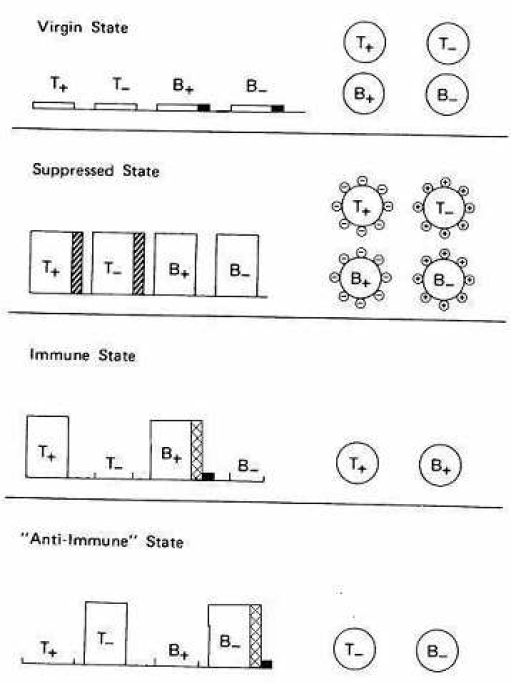
\includegraphics[scale=0.6] {img/symmetrical_network_theory.png}
    \caption{The model of the symmetrical network theory}
\end{figure}
\par
In order to make the problem easy to understand, it is assumed that only two main types of lymphocytes respond to specific antigen attacks[7]. The first group is positive set or collection of antibody which is called antigen-binding, with T+ and B+ respectively representing T cells and B cells, this type of cell has an idiotype and can recognize an antigen, binds and reacts with the antigen. The second is negative set or anti-idiotype set, with T- and B- representing anti-idiotype T cells and B cells, respectively, and cells in this class can recognize idiotype. Receptors in the anti-idiotype set correspond to receptors in the V region of the antibody collection. There are three interactive forms between the two sets, namely stimulation, suppression and killing. When two types of lymphocytes meet, stimulation occurs and the receptors are cross-linked. If a class of lymphocyte (+) receptors can be cross-linked with another type of lymphocyte (-) receptor, the opposite can also be connected, so bi-directional symmetric stimulation behavior can occur between the two sets. The inhibitory behavior between the two cell types is due to the blockade of specific T cell factor receptors. The T cell factor molecule is identical to the receptor and has only one V region. They inhibit receptors but do not cross-link receptors. The positive factor can prevent the negative set of receptors, and the negative factor can also block the positive set of receptors, so the inhibition behavior also has a symmetrical relationship. Finally, if antibodies with specificity A can kill specific B cells, antibodies with specificity B will also kill specific A cells. That is, the immune system has symmetry.
\par
From the symmetric network, it can be seen that the four stable states of the system including T+, B+, T-, and B- cells are the initial state, the inhibitory state, the immune state, and the anti-immune state, as shown in FiIG.5:
\begin{itemize} 
\item
 The initial state is a symmetrical state in which the number of cells in the positive and negative collections is small. The positive collection of cell antibodies kills the negative collection cells, and the negative collection of cellular antibodies kills the positive collection cells, that is, continuously kill each other. 
\item
In the inhibitory state, the number of cells in positive and negative collections constantly increases, which is mainly affected by the inhibitory effect of T cell factors. 
\item
In the immune state, the number of cells in the positive set is large, and the antibody in the positive set eliminates negative cells, which is a response state in terms of antigen stimulation, because positive cells are no longer limited by the number of negative cells. 
\item
 In the anti-immune state, the negative set of cellular antibodies eliminate the cells in the positive set, which is the reverse state of the immune state, and thus is the reversed response state.
\end{itemize}

\section{5. The environmental detection algorithm}
The environmental detection algorithm proposed in this paper, based on the biological immune theory, introduces the function of T cells into the detection algorithm, and proposes a detection algorithm based on the B-T cell immune network formula, which is more in line with the actual operating mechanism of the immune system. This reduces the randomness of the algorithm based on the B-cell immune network formula detection and improves the efficiency of multi-robot cooperative detection.
\par
There are many ways to describe the robot's environment. Since the grid method is more suitable for processing sonar sensor data, and the grid method is easy to create and maintain, the spatial expression consistency is good. Therefore, the grid method is used to establish the environment map. The environment the robot is to detect is divided into a series of squares. Each square is uniquely determined by the abscissa and ordinate. Both robots and unknown obstacles occupy a square in an unknown environment, and each step of the robot reaches a grid.
\par
Each grid has a state parameter P that indicates whether it is occupied or not. Parameters have two state values: Occupied and Idle. Before being detected, when there is no knowledge of the environment, there is no prior knowledge. The probability of being occupied or idle is the same, ie, P (occupancy) = 0.5, P (idle) = 0.5. When the robot probes, the probability of occupation or freeness of the grid is updated according to the Bayesian rule; Whether the grid has been probed, the program adds a state parameter S to whether or not the grid is detected. It has two state values: detected and undetected; S(i, j)=-1 indicates (i, j) The grid of the position is not detected, ie S(i, j)=0 indicates that the grid at the (i, j) position has been detected by other robots.

\subsection{5.1. Robot Antigen Information}
The detection points of multiple robots in the environment to be probed can be randomly distributed. After the detection starts, the robots simultaneously and autonomously detect and scatter the detection as much as possible. The robot always uses the boundary point as its own detection target, continuously known to the unknown. The field is probed and eventually fully explored. The boundary point is the boundary point between the detected environment and the undetected environment. At the beginning, the perimeter is all border points. As the detection area gradually increases, the boundary point area also expands. When the environment is gradually detected, the unknown areas are getting smaller and the boundary points are getting less and less. Finally, boundary point disappears completely, that is, the detection is completed.
\par
The local environment sensed by the robot is equivalent to the antigen in the immune system. The antigen information includes which grids are occupied and which grids have been detected in the environment detected by the robot.
\par
The robot has a movable grid in the environment, as shown in FIG.6:
\begin{figure}
\centering
    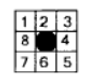
\includegraphics[scale=0.9] {img/movement_direction.png}
    \caption{The robot's direction of movement}
\end{figure}
\par
The black dots in the figure are robots. The surrounding grids are arranged in a sequence to be moved. They represent the 8 antibodies produced by the robot (B cells). The matching rate \boldmath$g_{i}$ between these antibodies and the antigen is taken into consideration of the cost paid for and the gains obtained by selecting the antibody (cell to be selected). According to the state of the surrounding grid, the \boldmath$g_{i}$ value in the following formula(5.1) is calculated as follows:
\begin{equation}{
    g_{i}=\frac{1}{(k_{1}\cdot expense+k_{2}\cdot occupy+k_{3}\cdot gain+1)}}
\end{equation}
\par
Among them, i=1-8. Indicates the price paid by the robot to detect the next grid from its grid. If the surrounding grid is undetected, that is \boldmath$S_{i}$=-1, then the expense is 0, if the surrounding grid has been detected, that is, \boldmath$S_{i}$=0, the expense is 1, their values represent if a surrounding If the grid has been probed, the corresponding expense takes a large value, making \boldmath$g_{i}$ smaller, thus discouraging the robot from selecting this grid. Occupy represents another type of cost that the robot will take to detect the next raster from its grid. Occupy is set to 1 if the surrounding grid has an obstacle \boldmath$p_{i}$=1. If the surrounding grid has no obstacle \boldmath$p_{i}$=0 and the accident is set to 0, its value setting indicates that if the surrounding grid has obstacles, occupying a larger value will make \boldmath$g_{i}$ smaller, so it is possible to avoid the robot from selecting this grid. Gain represents the gain obtained after reaching the next target raster, which is a blank area that can continue to be probed.
\par
In the detection environment, the robot must not only pay attention to its own local environment, but also cooperate with other robots to quickly complete a full-scale exploration task. From the perspective of global detection, multiple robots are best able to detect in a decentralized manner and avoid crowding to one place. Therefore, robots need cooperation and communication to exchange information so that they can each detect in the opposite direction. In the immune algorithm, this cooperative relationship between robots manifests itself as the interaction between antibodies. As shown in Figure 5-2, the coordinates of the robot R1 are (x1, y1), the coordinates of the robot R2 are (x2, y2), and the interaction coefficient between the antibody generated by R2 and the antibody i of R1 is set to mi2, respectively. i=1-8, i corresponds to the surrounding eight grids, and R1R2 indicates the direction of force applied by R2 to R1.
\begin{figure}
\centering
    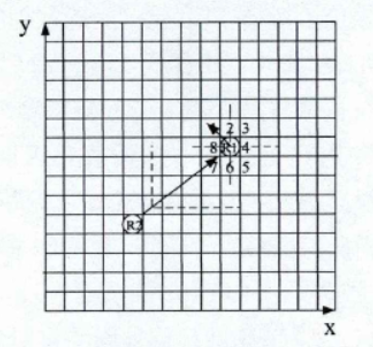
\includegraphics[scale=0.6] {img/immune_network_force_diagram.png}
    \caption{Robot force diagram}
\end{figure}
\par
Since the next detection of the robot R1 has eight neighboring cells to be selected, that is, eight antibodies generated by the B cells, the vector direction (antibody direction) of the robot R1 pointing to the neighboring grid can be orthogonally decomposed into four positive and negative directions. In one or both of the cross directions, R2R1 may also be orthogonally decomposed into one or two of the orthogonal directions. If the antibody and R2R1 are completely in the same direction after they are decomposed, the antibody is said to be in full compliance with the R2R1 direction if orthogonal decomposition occurs. In the backward direction, only one direction is the same, and in the other direction, the antibody portion is said to conform to the R2R1 direction. If both directions are reversed, the antibody is said to not conform to the R2R1 direction. From FIG.7, it can be seen that antibodies 2, 3, and 4 fully conform to the R2R1 orientation, antibodies 1 and 5 conform to the R2R1 orientation, and antibodies 6, 7, and 8 do not conform to the R2R1 orientation. We hope that the R1 and R2 robots will work in parallel and select different targets at the same time to perform parallel detection. Therefore, if the antibodies generated by the R1 robot fully comply with the R2R1 direction, the antibodies of the robot R2 will stimulate the antibodies against the R1 and have the largest excitation value; if partially The antibody of R2 from robot R2 also stimulates the antibody against R1, but the stimulus value is slightly lower; if it does not, the inhibition occurs.

\subsection{5.2. Detection algorithm flow}
Each of the robots detects the environment in accordance with the following procedure to form a fully distributed detection system similar to the immune system.
\par
Step 1: set the robot, object, obstacle position.
\par
Step 2: The robot senses the local environment from the current position and determines whether all the surrounding points are obstacles or have been detected. If yes, go to the seventh step; otherwise, enter the third step.
\par
Step 3: Generate antibodies to the surrounding eight grids, and calculate the matching ratio gi between antibody i and antigen according to formula (3). If there is a maximum gi value, select the grid corresponding to the antibody with the highest matching rate gi as Next, probe the grid and go to the fourth step; if there is more than one gi, go to the fifth step.
\par
Step 4: The selected grid is used as the next detection target. The robot moves one step to the selected grid and then back to the second step to continue the detection.
\par
Step 5: When multiple values are the same, first calculate the affinity or rejection coefficient between antibodies, consider the role of other robots (B cells) in the communication range for each antibody of the robot; then calculate the level of antibody i adaptation if present The maximum value, select its corresponding grid, as the next probe grid, back to the fourth step; if there are multiple values are the same, go to the sixth step.
\par
Step 6: Calculate the cell concentration, consider the cell's regulatory effect on each antibody of the robot; calculate the excitation level Si(t) of the antibody i, and finally select the antibody with the highest concentration. The grid corresponding to the antibody is the direction of movement of the robot. The smallest grid of corners, go to the fourth step.
\par
Step 7: The robot selects the boundary point for detection. If there is no boundary point, it means that all the detections have been completed and the detection ends.
\begin{figure}
\centering
     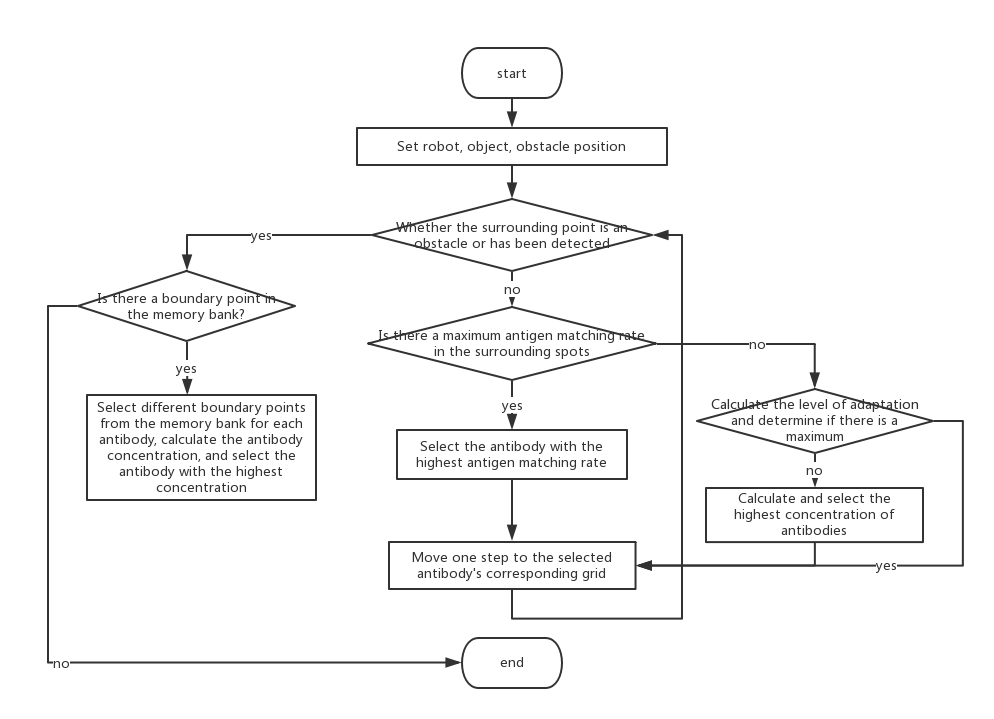
\includegraphics[scale=0.40] {img/immune_network_flowchat.png}
    \caption{Environmental detection flow chart}
\end{figure}

\subsection{5.3. Algorithm experimental results}
FIG.9 is a detection roadmap based on this detection algorithm. The number of grids in the simulation environment is 20*20. The robot does not know the environmental status. It obtains external data by real-time detection and communication, and decides its own next grid according to the immune algorithm. position. The black convex objects and L-shaped objects in the environment indicate the grid occupied by the obstacles. The robot is represented by a circle number and placed in the initial position. The three line types represent the detection routes of the three robots starting from the initial position.
\par
In order to check whether the robots can cooperate effectively, arrange 3 robots to enter the lower left corner of the environment to be detected. As can be seen from the route in the figure, the robot detects the environment in a decentralized way. Firstly, the robot No. 3 moves to the right. The robot No. 2 moves the left-to-right direction of the second step in the third step. The principle followed is the gi calculation formula. The meaning of the expression is to select the grid with fewer detectable points around it as the target of the next detection. According to this method selection, it can be ensured that the areas detected by the robot are connected one by one, and the missing places are minimized. Then, the number of times that the robot will make up and miss leaks will be small, which will increase detection efficiency.
\par
When robot No. 1 walks to the (1,20) grid, the surroundings are surrounded by the environmental edges and the detected grid. At this time, the robot can only find the optimal boundary point for detection, and the route to the boundary point appears. Repeated detection. It can be seen from the figure that when the (9,14) grid is detected, the two robots repeat the detection again. The whole graph shows that the robots have effectively cooperated with each other, and the complete detection of the unknown environment has been efficiently achieved. The robot detection coverage rate has reached 100 percent. When selecting the next detection target, the obstacle avoidance is well achieved.
\begin{figure}
\centering
    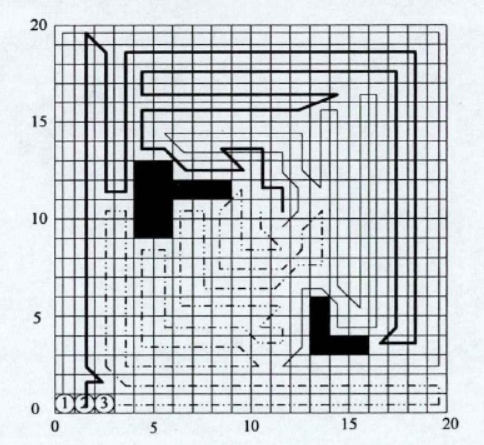
\includegraphics[scale=0.50] {img/immune_network_route_map.png}
    \caption{Exploration Roadmap}
\end{figure}

\section{REFERENCES}
\noindent
[1] 1N. K. Jerne (1974) Towards a Network Theory of the Immune System, Ann. Immunol. (Inst. Pasteur), 125C, 373-389.
\par
\noindent 
[2] N. K.Jerne (July 1973) Scientific American pp. 49-57. 
\par
\noindent
[3] N. K. Jerne (1974) Clonal selection in a lymphocyte network. In Cellular Selection and Regulation in the Immune Response, Edelman, G. M. ed, Raven Press, New York, op. cit. p. 39-48.
\par
\noindent
[4] N. K. Jerne, J. Roland and P.-A. Cazenave (1982) Recurrent idiotopes and internal images. EMBO J. 1, 243-247.
\par
\noindent
[5] P. H. Richter (1975) A network theory of the immune response. Eur. J. Immunol., 5, 350-354.
\par
\noindent
[6] G. W. Hoffmann (1975) “A network theory of the immune system.” Eur. J. Immunol., 5, 638-647, 1975.
\par
\noindent
[7] G. W. Hoffmann. A neural network model based on the analogy with the immune system [J]. Theoretical Biology, 1986, 122:33-67.

\end{document}
